\documentclass[12pt,a4paper]{report}
\usepackage{graphicx}
\usepackage{blindtext}
\usepackage[utf8]{inputenc}
\usepackage[hidelinks]{hyperref}
\usepackage{indentfirst}
\usepackage[printonlyused]{acronym}
 
\begin{document}


\begin{titlepage}
	\centering
	{\scshape\Large Czech Technical University in Prague\par}
	\vspace{0.3cm}
	{\scshape\large Faculty of Information Technology\par}
	\vspace{0.3cm}
	{\scshape Department of software engineering\par}
	\vspace{1cm}
	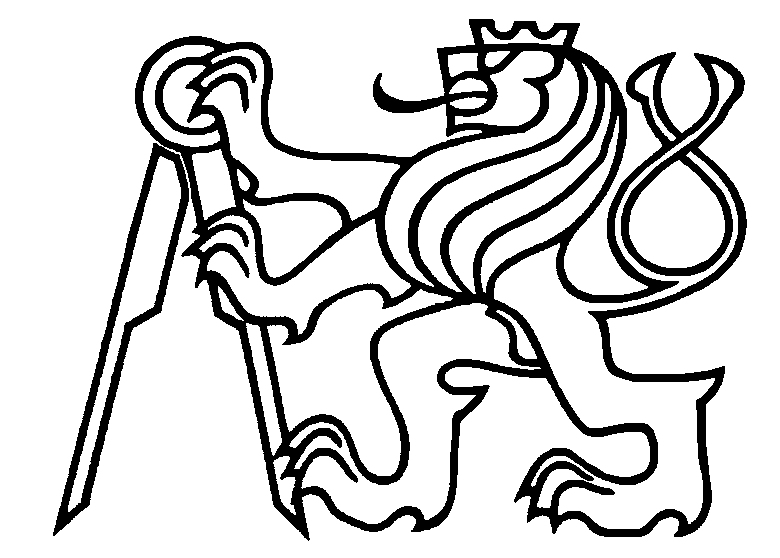
\includegraphics[scale=0.3]{cvut.png}\par
	\vspace{2cm}
	{\scshape\LARGE Positional report\par}
	\vspace{1cm}
	{\Large\bfseries Back-end API and payments system for crowdfunding platform ElateMe\par}
	\vspace{3cm}
	{\large\itshape Kuzmovych Yevhen\par}
	\vfill
	supervised by\par
	Ing.~Jiří \textsc{Chludil}
	\vfill

	{\large December 11, 2016\par}
\end{titlepage}



% Table of contens

\tableofcontents
\renewcommand{\thesection}{\arabic{section}}

\vfill

\section*{Keyword}
ElateMe, crowdfunding platform, social network, back-end API, DBMS, RESTful

\newpage
\section*{List of Acronyms}
\begin{acronym}
	\acro{API}{application programming interface}
	\acro{MVC}{model-view-controller}
	\acro{DBMS}{database management system}
	\acro{REST}{Representational state transfer}
\end{acronym}


\section{Introduction}
 
ElateMe is a new crowdfunding platform with elements of the social network. Unlike other similar projects like Kickstarter or Patreon that help bring creative, commercial projects to life by means of  interested people, ElateMe is focused on fulfillment of personal wishes with the help of users’ friends. The user can create a wish and set its cost, title, and a short description. His friends then will be able to contribute to his wish by donating money. When wish gathers needed amount, money will be transferred to the user bank account. The social part of the application is providing an ability for the user to subscribe to his friends, communicate with other users, rate and comment others’ wishes. \par
The aim of this thesis is to analyze functional, nonfunctional requirements and use cases of the project, design database model and server architecture, implement back-end \ac{API} and payments system for this service.



\section{Existing solutions}

There are many examples of crowdfunding platforms and social networks. But ElateMe is a new concept that combines them both. So there is no exact solution for such system. Yet in this report, popular crowdfunding platforms and social networks will be considered as existing solution. Their stack of technologies can be taken as an example and adjusted for needs of this project.



\section{Possibilities of the solution}

The back-end is part of the application that contains its business logic, processes its data in the database and provides \ac{API} for the client side of application (front-end). The main task of back-end developer on initial stage is to select back-end technology stack, therefore, programming language, corresponding web framework and \ac{DBMS}.

	\subsection{Programming language}
Choice of programming language leads to the choice of the corresponding web framework. It is crucial to choose technology that allows a developer to produce a working solution, supports scalability and flexibility for future modifications and extensions and allows to write elegant, readable and debuggable code.\par
The most common programming languages and frameworks for web development are (examples of usage were taken from StackShare\cite{stackshare}):

\begin{itemize}
	\item Ruby and Rails (Kickstarter, Twitter)
	\item Python and Flask (Patreon) or Django (Instagram)
\end{itemize}

Ruby is open source,  interpreted, object-oriented programming language. It is widely used in web programming. Rails serves as a web framework for the Ruby language. It’s used by companies ranging from small start-ups to large enterprises. Ruby on Rails is a great framework for quick prototyping but it can be too slow for large-scale applications. \par
Python is an interpreted, object-oriented, high-level programming language. Its syntax is simple that makes code written in Python easy to read and understand. It has two main web frameworks that are used by such companies as Patreon, Instagram, Google, Snapchat, and others.


	\subsection{DBMS}
	
Another important part of the technology stack is the database and its \ac{DBMS}. Considering the fact that structure of this application is highly dependent on data, its integrity, scalability, and security, choice of appropriate \ac{DBMS} is essential. The most used databases in web development are:

\begin{itemize}
	\item MySQL (Kickstarter, Patreon, Twitter, Facebook)
	\item PostgreSQL (Instagram)
	\item SQLite
\end{itemize}

SQLite is self-contained, file-based database. It is simple to install and set up. SQLite is often used for debugging purposes as a temporary database.\par
MySQL and PostgreSQL are the most popular \ac{DBMS}s for web development. They both offer a lot of functionality to the users. As the standalone database servers, MySQL and PostgreSQL provide powerful interfaces for applications to communicate through.



\section{Chosen methods}

Taken into consideration everything mentioned above and authors own experience and preferences it was decided to use Python as a programming language, Django as a web framework and PostgreSQL as \ac{DBMS}.


	\subsection{Python}
	
Python will be a base of the server. It was chosen as a primary programming language because it was designed to be simple and highly readable which is very important for large-scale projects. Its syntax and standard library simplify and speed up a development.\par
The first version of basic back-end \ac{API} for ElateMe is expected to be ready at the end of January 2017. So fast prototyping is a required option for chosen programming language. That is why Python is the best fit for purposes of this project.

	
	\subsection{Django}

Django\cite{django} is open source web framework for python. It provides a high level abstraction of common web development patterns. It follows \ac{MVC} design pattern. Django uses \ac{MVC} to separate model a data and a business logic of application, view a representation of the information for the user, in this case, the client side of application and controller a an interface of the application, in this case, set of URLs to communicate with front-end.

	
	\subsection{Django REST framework}
	
\ac{REST}\cite{rest} is the architectural solution for the transfer of structural data between server and client. It is a broad topic and will not be described in this report. Authors knowledge of \ac{REST} comes from \textit{Design solutions for SOAP/WSDL and RESTful web services} by Robert Daigneau\cite{rest}.\par
Django REST framework is open source tool built on Django framework. It contains needed tools for implementation of \ac{REST}ful \ac{API} and follows all constraints of \ac{REST}ful server mentioned in \cite{rest}.

	
	\subsection{PostgreSQL}

On initial stage of the development, SQLite will be used as a \ac{DBMS}, because it does not require a standalone database server and is simple to set up. The database will be changed and migrated to PostgreSQL later.\par
PostgreSQL\cite{postgres} is powerful, open source relational \ac{DBMS}. It has advanced features such as full atomicity, consistency, isolation, durability. Django framework provides great \ac{API} for working with PostgreSQL databases.
	


\section{Current project state}

At the moment the project is at the stage of development. Main business processes, requirements, use cases were analyzed and documented. On back-end side, basic \ac{API} for user authentication with facebook account and for wishes management has been implemented. On front-end side, there is complete client architecture and partial implementation of the application interface.
Next step of development will be studying of online payment systems, a continuation of work on server \ac{API}, and testing.



\section{Conclusion and future outlook}

The output of this bachelor thesis will be the analysis of business processes, requirements and use cases of ElateMe project, implemented back-end interface for the client-server communication, the online payment systems for donations. The main goal for the author though is to analyze and learn tools for web back-end development such as Python programming language and Django web framework, practice building complicated systems using them, learn to design server architecture and explore various online payment systems.\par
It is expected to have the working version of the application and its release at the end of academic year 2016/2017. Android and iOS versions of the mobile application will be uploaded to Google Play and Apple Store respectively. There is a possible continuation of work and support of the project in case of successful release and advertising campaign.



\renewcommand\bibname{References}
\begin{thebibliography}{9}
	
	\bibitem{stackshare}
StackShare. \emph{StackShare} [online]. [Accessed 9 December 2016]. Available from: https://stackshare.io/

	\bibitem{django}
HOLOVATY, Adrian and Jacob. KAPLAN-MOSS. \emph{The definitive guide to Django: Web development done right}. 2nd ed. Berkeley: Apress, c2009. Expert's voice in Web development. ISBN 978-1-4302-1936-1.
	
	\bibitem{rest}
DAIGNEAU, Robert. \emph{Service design patterns: fundamental design solutions for SOAP/WSDL and RESTful web services}. Upper Saddle River: Addison-Wesley, c2012. Addison-Wesley signature series. ISBN 978-0-321-54420-9.

	\bibitem{postgres}
OBE, Regina O. and Leo S. HSU. \emph{PostgreSQL: up and running}. Sebastopol: O'Reilly, c2012. ISBN 978-1-449-32633-3.

\end{thebibliography}

 
\end{document}